\documentclass[10pt]{article}

\usepackage{fixme}
\fxsetup{ status=draft, layout=inline}
\usepackage[pdftex]{graphicx}

\ExecuteOptions{letterpaper,10pt,twocolumn,oneside,final,journal}

\begin{document}
The \fxnote{a word for ``more and more popular''} social media websites 
collect a huge amount of latent visual information for environmental and ecology monitoring.
In this work, we propose to reconstruct satellite maps of ecology status 
across North America continent 
through 12 million publicly available geo-temporal tagged images.
We select snowfall and greenary vegetation coverage as important ecology phenomena with satellite 
maps available to compare with, and straight forward \fxnote{I just want to say easy.} to identify by human. 
First we examine the existance of snow and greenery respectively on all the images and 
aggregate this result according to the geo and 
temporal attributes to make continental scale prediction over each time period. 
Then we compare our results with satellite maps for each phenomenon and find that we fill the blanket 
when satellites failed to get any data at very cloudy area or when satellite data is too 
coarse to small changes \fxnote{like vegetation case, satellite data miss data at almost all of 
the transition period}. In this case, our results are very helpful for ecologists especially when 
the data during changing or transition period is all they need without a better way to find. \fxnote{is this clear?}
We also conduct experiments with fixed time or location and find our result 
as a promising complementary of satellite maps. Moreover, we also compare the performance based on visual evidence and textual mining. 
It turns out tags can describe snowfall very well but due to \fxnote{misleading of words describing 
vegetation}, it works less satisfactory on vegetation coverage estimation.

\section{Introduction}

Monitoring the state of the natural world is a key challenge of
ecological and biological research, since predicting future changes
depends on accurate observations of the present. Satellites give
observations at large scale but can only be applied to phenomena that
can be seen from far above, and are limited by cloud cover and other
atmospheric conditions.  Citizen science projects~\cite{citizensci} can
produce quality data, but require significant incentives to encourage
participation over large scale areas, and clever designs to derive
accurate data from untrained observers.  A potentially rich
alternative is to mine publicly-available social media for
observations relevant to natural world, in effect turning the billions
of social media users into citizen scientists without any explicit
actions on their part.  This idea is motivated by the large amount of
work that has  mined social media  to predict and
observe properties of the real world, including the stock
market~\cite{bollen11twitter},
elections~\cite{you2015multifacetedelections}, tourism
activity~\cite{wood2013usingtourism}, and so on.

However, most of this work has used textual data like Facebook posts
and Twitter feeds.  Social images are potentially a richer source of
information because they often include incidental evidence about the
natural world (Figure~\ref{fig:flickrexp}).  In addition, they record
visual documentation that can later be analyzed, inspected, and
validated; the danger of relying on text analysis and the importance
of validation was recently recently illustrated by the case of Google
Flu, which initially showed great promise in monitoring the spread of
influenza by mining search engine queries~\cite{ginsberg09flu}, but
was later found to be largely inaccurate~\cite{lazer2014parable}.
Of course, a key challenge in mining images is how to extract useful
semantic information.

\begin{figure}[t]
{\tiny{
\begin{center}
\begin{tabular}{@{}c@{\,\,\,}c@{\,\,\,}c@{\,\,\,}c@{\,\,\,}c@{\,\,\,}c@{\,\,\,}c@{\,\,\,}c@{\,\,\,}}
%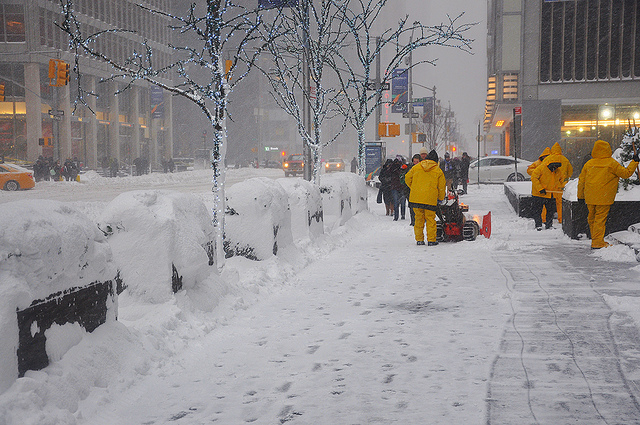
\includegraphics[width=0.12\textwidth]{image/citysnow.jpg} &
%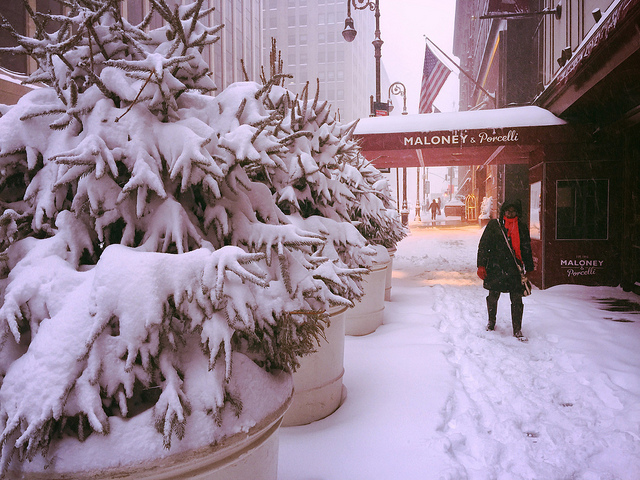
\includegraphics[width=0.1\textwidth]{image/citysnow2.jpg} &
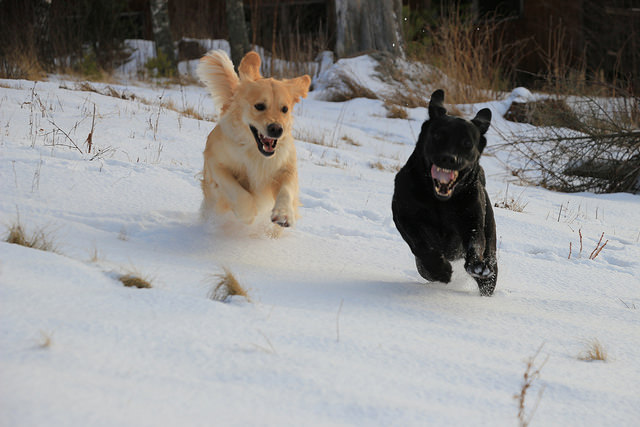
\includegraphics[width=0.15\textwidth,height=0.75in]{image/dogsnow.jpg} &
%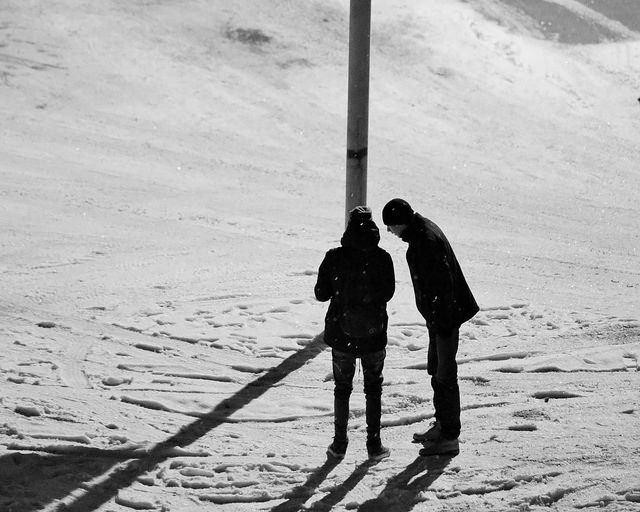
\includegraphics[width=0.1\textwidth]{image/humansnow.jpg} \\
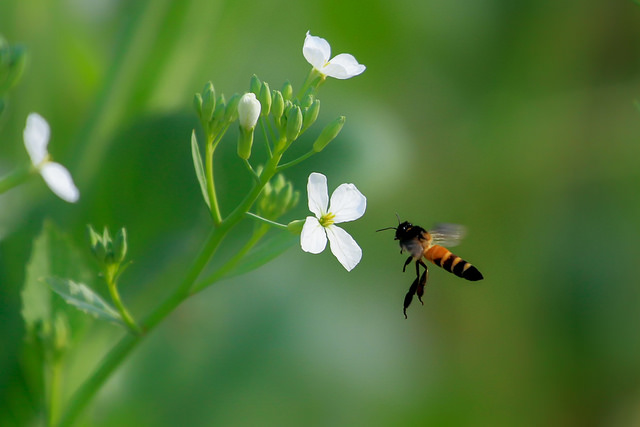
\includegraphics[width=0.15\textwidth,height=0.75in]{image/intentiongreen.jpg} &
%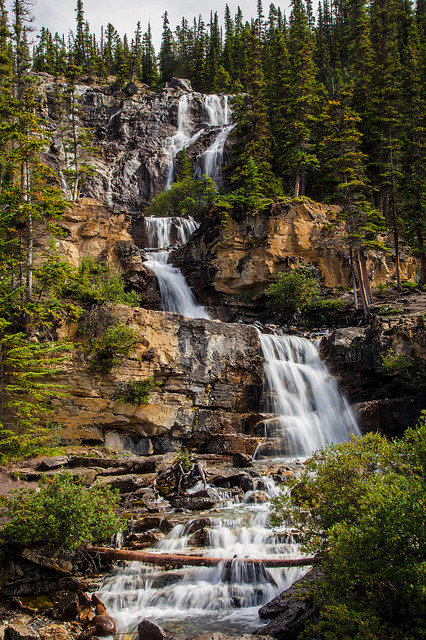
\includegraphics[width=0.1\textwidth]{image/waterfallgreen.jpg} &
%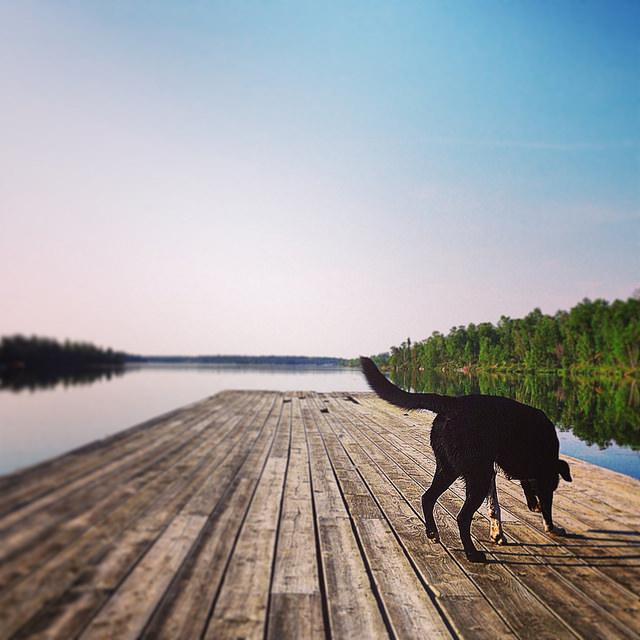
\includegraphics[width=0.12\textwidth,trim=0 0 0 cm,clip]{image/dogtree.jpg} &
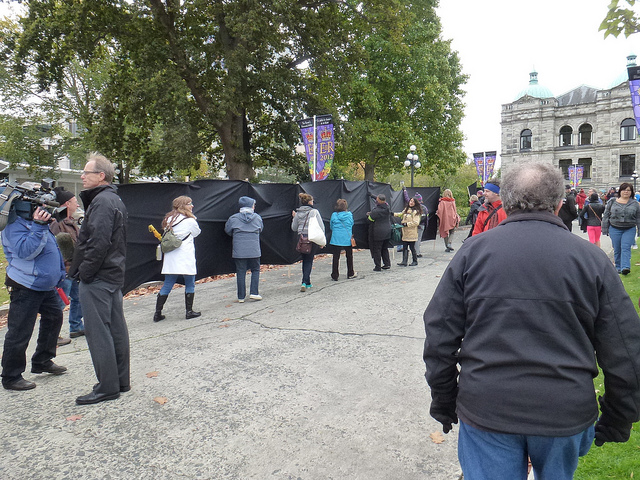
\includegraphics[width=0.15\textwidth,height=0.75in]{image/humantree.jpg} \\
\end{tabular}
\end{center}
}}
\vspace{-12pt}
\caption{Many social media images capture information about the state of the natural world, both intentionally or incidentally.}
\label{fig:flickrexp}
\vspace{-12pt}
\end{figure}


A few papers have begun to apply computer images for environmental
properties, including temperature~\cite{glasner2015hot}, cloud
cover~\cite{murdock2013webcam2satellite}, and smog conditions~\cite{li2015smog}. Most of
these papers use video data (e.g.\ from static webcams) so that visual
changes over time can be easily detected. Video camera feeds are
potentially very useful for studying longitudinal changes across time
in one particular place, but are limited to studying places where
cameras have been installed. Social photo sharing websites potentially
represent a complementary source of data, that give much greater
spatial coverage: whenever a user takes a photo at a particular place
and time and uploads it to Flickr, they are contributing a potentially
useful observation.

In this paper, we test the feasibility of leveraging these noisy and
biased images as a new source to observe nature, using modern deep
learning-based computer vision algorithms to recognize image content
automatically.  As a case study, we investigate two particular
phenomena, snowfall and vegetation coverage, since they are important
properties of the environment, they are relatively easy to recognize,
occur frequently in social images, and have satellite maps available
to serve as ground truth. This choice was also inspired by Fedorov et
al~\cite{fedorov2015snowwatch,fedorov2014snow}, who use video analysis
to monitor snow fall on mountains, and Zhang et
al~\cite{ecology2012www}, who predict snowfall from image collections
but using text tag analysis.  We first collect image data labeled to
reflect the presence of absence of ecology phenomena, and train
classifiers using Convolutional Neural Networks to recognize these
ecology phenomena in individual images. Of course, these classifiers
are noisy, and social image data is noisy also, with many inaccurate
timestamps and geo-tags.  We thus train an additional classifier that
examines all images taken at a given place and time, runs the image
classifier on each one, and then predicts if the phenomena actually
occured there and then.  Finally, we evaluate at a large scale,
training and testing on millions of Flickr images and quantiatively
evaluating the performance at hundreds of thousands of places and
times.

%% Inspried by an earlier work~\cite{ecology2012www} 
%% %\fxnote{ Fixed: cite{www}} 
%% analyzing ecology phenomenon from image tags only. We apply a new approach by 
%% understanding visual content of images, and run experiments on the exact same 
%% data set to study how vision techniques could help in social media data mining 
%% compared to using textual data alone. Also, to our best knowledge, among all the 
%% research works performing social sensing with image data, this is the first one 
%% providing continental scale quantitative performance evaluation.










\begin{figure}[t]
\centering
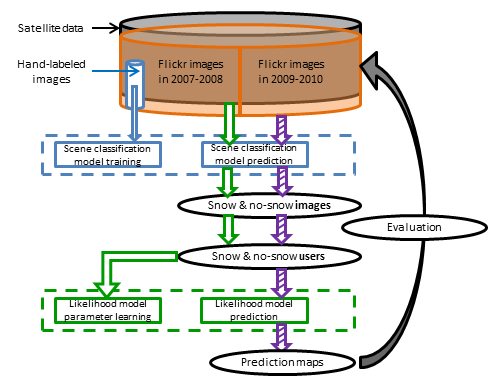
\includegraphics[scale=0.7]{figure/flowchartWevaluation.png}
\vspace{-12pt}
\caption{Overview of our approach. We train image classifiers(in blue) on large scale images. And by applying it to training images in 2007-2008, 
we train a likelihood model(in green) and finally make prediction by aggregating these visual evidence.}
% \fxnote{first classifier, then prediction}
\label{fig:overview}
\vspace{-12pt}
\end{figure}


%\section{Related work}
In last few years, crowd-sourcing data from social media 
as a large scale and free to public data source
has \fxnote{received lots of attention from; or (become more and more popular to)} 
researchers working on using textual contents to
predict elections~\cite{you2015multifacetedelections},
using geo-tags to quantify
tourism in nature area using geo-tag profile of social media users ~\cite{wood2013usingtourism},
\fxnote{talk a lot about motivation of scientific report paper since it's in nature area}
to draw coastline~\cite{omori2014can}~\cite{Can geo-tags on flickr draw coastlines?}, 
using geo and temporal tags to analyze people's event-based activity when large group of people gathering together during a function of time such as football match,
and using both geo and textual tags to 
extract land use information from Panoramio~\cite{vsecerov2015analysis} ~\cite{Analysis of panoramio photo tags in order to extract land use information, Towards Better Land Cover Classification Using Geo-tagged Photographs},
in~\cite{ecology2012www} \fxnote{cite{www}}, Zhang \etal estimates \fixme{missing letter in compiling} snowfall and vegetation coverage 
based on geo, temporal and textual tags of Flickr images. \fxnote{accuracy of geo-temporal problem, and now it's getting better.}

Since public-sharing photos provides such a huge potential in social and environmental study, it's 
natural to see a lot of works start analyzing image contents. Webcam providing dense temporal images 
is a good source to monitor the nature. A series of works explore sequences 
of webcam images describing outdoor scene with 40 transient attributes~\cite{transattri}, estimating dynamic cloud maps ~\cite{murdock2015building, murdock}, exploring interactions between visual elements and the temperature \fxnote{or just as the title: exploring correlations between appearance and temperature} ~\cite{hot or not}, and monitoring the dynamic snow phenomena at mountain areas ~\cite{fedorov2015snowwatch, fedorov2014snow}. 
To evaluate the study of temperature, cloud, and snowfall amount,
 researchers can easily compare their results with satellite maps. 
Some works also use crowd-sourcing data from other sources, for example, Google street view provides selectively dense geo distributed images to help navigating the environment ~\cite{khosla2014looking} and understanding urban scene and predicting urban perception ~\cite{porzi2015predicting}, and Li \etal use the co-occurrence statistics of celebrities appears on news images to auto tag photographs of celebrity community ~\cite{li2015celebritynet}
\fxnote{give a term like social identity?}. 
Unfortunately, 
the evaluation in these works are either not in continental scale or just via quality visualization.
Performance of social activity studies, on the other hand, are even harder to evaluate.
\fxnote{say more about our evaluation? or move this to another place?}

Flickr and Panoramio as very popular photo-sharing websites 
``involuntarily'' support researchers identifying salient city attributes and analyzing the visual similarity among different cities in order to apply computer vision to urban planning ~\cite{zhou2014recognizing}
Photo-sharing websites collecting visual contents directly from people's activity and their surrounding areas which is so important, hard to collect otherwise but also very noisy. \fxnote{write something about so there are very few work appears and so we are working on this?}

%\fxnote{not sure about keeping this paragraph or not. it seems duplicate of the 2 paragraphs above}

The fact that webcam can only be placed far away from people 
 makes it almost impossible to monitor people's activity, even not the surrounding area close to
residential or \fxnote{crowd? I mean groups of people like downtown, not ski activity but like people 
going to work and back everyday also a good topic to use temporal dense images but Webcam is not good 
at this.} Social media, on the other hand, provides a larger freedom on location distribution. 
In fact, as a complementary, almost all the photos shared online are from locations people usually go to. 
\fxnote{how helpful is this to study more areas close to urban planning, market sharing, everyday living,
anything related to people}

Our work take the advantage of studying ecology phenomena with \fxnote{easy to get, more reliable} satellite maps as
 ground truth and use social media data to \fxnote{monitor? insight?} these information from \fxnote{
locations more related to people}. We provide continental scale quantitative evaluation and introduce our
 method to tackle the problem of noisy and biased data, in order to support extended studies in other areas. \fxnote{just want to say more areas in natural or not only natural but also social}




\end{document}